\documentclass[12pt, titlepage]{article}

\usepackage{fullpage}
\usepackage[round]{natbib}
\usepackage{multirow}
\usepackage{booktabs}
\usepackage{tabularx}
\usepackage{graphicx}
\usepackage{float}
\usepackage{hyperref}
\usepackage{soul}
\hypersetup{ colorlinks, citecolor=blue, filecolor=black, linkcolor=red,
    urlcolor=blue }

\input{../../Comments}
\input{../../Common}

\newcounter{acnum}
\newcommand{\actheacnum}{AC\theacnum}
\newcommand{\acref}[1]{AC\ref{#1}}

\newcounter{ucnum}
\newcommand{\uctheucnum}{UC\theucnum}
\newcommand{\uref}[1]{UC\ref{#1}}

\newcounter{mnum}
\newcommand{\mthemnum}{M\themnum}
\newcommand{\mref}[1]{M\ref{#1}}

\begin{document}

\title{Module Guide for \progname{}} 
\author{\authname}
\date{\today}

\maketitle

\pagenumbering{roman}

\section{Revision History}

\begin{tabularx}{\textwidth}{p{3cm}p{2cm}X} \toprule {\bf Date} & {\bf Version}
& {\bf Notes}\\
\midrule
Jan 18, 2023 & 1.0 & Revision 0\\
\midrule
\color{red}{Apr 3, 2023} & \color{red}{1.1} & \color{red}{Revision 1}\\
\bottomrule
\end{tabularx}

\newpage

\section{Reference Material}

This section records information for easy reference.

\subsection{Abbreviations and Acronyms}
See SRS Documentation at
\href{https://github.com/parkd-app/park-d/blob/main/docs/SRS/SRS.pdf}{Park'd
Software Requirements Specification}.\\

\noindent
\renewcommand{\arraystretch}{1.2}
\begin{tabular}{l l} 
  \toprule		
  \textbf{symbol} & \textbf{description}\\
  \midrule 
  \progname & Parking Lot Application\\
  AC & Anticipated Change\\
  DAG & Directed Acyclic Graph \\
  M & Module \\
  MG & Module Guide \\
  OS & Operating System \\
  R & Requirement\\
  SC & Scientific Computing \\
  SRS & Software Requirements Specification\\
  \progname & Explanation of program name\\
  UC & Unlikely Change \\
  SUV & Sports Utility Vehicle \\
  RNN & Recurrent Neural Network \\
  ID & Identification\\
  \bottomrule
\end{tabular}\\

\newpage

\tableofcontents

\listoftables

\listoffigures

\newpage

\pagenumbering{arabic}

\section{Introduction}

Decomposing a system into modules is a commonly accepted approach to developing
software.  A module is a work assignment for a programmer or programming team.
We advocate a decomposition based on the principle of information hiding.  This
principle supports design for change, because the ``secrets'' that each module
hides represent likely future changes.  Design for change is valuable in SC,
where modifications are frequent, especially during initial development as the
solution space is explored.  

Our design follows the rules, as follows:
\begin{itemize}
\item System details that are likely to change independently should be the
  secrets of separate modules.
\item Each data structure is implemented in only one module.
\item Any other program that requires information stored in a module's data
  structures must obtain it by calling access programs belonging to that module.
\end{itemize}

After completing the first stage of the design, the Software Requirements
Specification (SRS), the Module Guide (MG) is developed. The MG specifies the
modular structure of the system and is intended to allow both designers and
maintainers to easily identify the parts of the software.  The potential readers
of this document are as follows:

\begin{itemize}
\item New project members: This document can be a guide for a new project member
  to easily understand the overall structure and quickly find the relevant
  modules they are searching for.
\item Maintainers: The hierarchical structure of the module guide improves the
  maintainers' understanding when they need to make changes to the system. It is
  important for a maintainer to update the relevant sections of the document
  after changes have been made.
\item Designers: Once the module guide has been written, it can be used to check
  for consistency, feasibility, and flexibility. Designers can verify the system
  in various ways, such as consistency among modules, feasibility of the
  decomposition, and flexibility of the design.
\end{itemize}

The rest of the document is organized as follows. Section \ref{SecChange} lists
the anticipated and unlikely changes of the software requirements. Section
\ref{SecMH} summarizes the module decomposition that was constructed according
to the likely changes. Section \ref{SecConnection} specifies the connections
between the software requirements and the modules. Section \ref{SecMD} gives a
detailed description of the modules. Section \ref{SecTM} includes two
traceability matrices. One checks the completeness of the design against the
requirements provided in the SRS. The other shows the relation between
anticipated changes and the modules. Section \ref{SecUse} describes the use
relation between modules.

\section{Anticipated and Unlikely Changes} \label{SecChange}

This section lists possible changes to the system. According to the likeliness
of the change, the possible changes are classified into two categories.
Anticipated changes are listed in Section \ref{SecAchange}, and unlikely changes
are listed in Section \ref{SecUchange}.

\subsection{Anticipated Changes} \label{SecAchange}

Anticipated changes are the source of the information that is to be hidden
inside the modules. Ideally, changing one of the anticipated changes will only
require changing the one module that hides the associated decision. The approach
adapted here is called design for change.

\begin{description}
\color{red}{
\item[\refstepcounter{acnum} \actheacnum \label{ac1}:] 
The type of vehicle information, such as the vehicle's length and width. This
may change to simply require the vehicle class, such as SUV or Utility vehicle,
using which the system would retrieve the dimensions.\\
\textbf{As of Revision 1, vehicle-related information is not used at all. In future revisions, this information will be collected and used to implement parking violation detection (single vehicle occupying multiple spots).}
}
\color{black}
\item[\refstepcounter{acnum} \actheacnum \label{ac2}:] The source of the video
footage (from a camera feed website or from a group member's device with a
camera)


\item[\refstepcounter{acnum} \actheacnum \label{ac3}:]{\color{red} The
implementation of machine learning model is subject to change(Different
generations of YOLO model may be used)\\
\textbf{As of Revision 1, YOLOV3 was eventually used in the project due to its
robustness that able to identify parking spots in any different footage angles.
In future revisions, different generations of YOLO architecture may be used to
provide even more accurate results }}


\item[\refstepcounter{acnum} \actheacnum \label{ac4}:] The layout of the parking
spaces and if they reflect the exact layout of the parking lot, or just
locations relative to one another.

\item[\refstepcounter{acnum} \actheacnum \label{ac5}:] Expand the stats of a
parking layout to include past stats and trends over a time period.

\item[\refstepcounter{acnum} \actheacnum \label{ac6}:] Extend the navigation to
start from outside the parking layout.

\item[\refstepcounter{acnum} \actheacnum \label{ac7}:] Represent the parking
layout in a more graphical way.

\end{description}

\subsection{Unlikely Changes} \label{SecUchange}

The module design should be as general as possible. However, a general system is
more complex. Sometimes this complexity is not necessary. Fixing some design
decisions at the system architecture stage can simplify the software design. If
these decision should later need to be changed, then many parts of the design
will potentially need to be modified. Hence, it is not intended that these
decisions will be changed.

\begin{description}
\color{red}{
\item[\refstepcounter{ucnum} \uctheucnum \label{ucIO}:] 
The type of information that is requested from the user to be provided to the
website in order to set tailored parking preferences (user ID, password and
vehicle information).\\
\textbf{As of Revision 1, vehicle information is not gathered from users. In future revisions, this information will be collected and used to implement parking violation detection (single vehicle occupying multiple spots).}
}
\color{black}
\item[\refstepcounter{ucnum} \uctheucnum \label{ucIO}:] Parking data will
continue to be generated from a remote back-end and relayed to the front-end.

\item[\refstepcounter{ucnum} \uctheucnum \label{ucIO}:] The application's main
goal is the efficient display of available parking spaces for a supported
parking lot.

\item[\refstepcounter{ucnum} \uctheucnum \label{ucData}:] The organization and
interfaces of the modules involved in representing a parking layout.

\item[\refstepcounter{ucnum} \uctheucnum \label{ucData}:] The parking status and
layout data will be stored in an agreed upon structure in json files.

\item[\refstepcounter{ucnum} \uctheucnum \label{ucIO}:] The Navigation Module
will give users directions to their selected parking spot.

\item[\refstepcounter{ucnum} \uctheucnum \label{ucIO}:] The Machine Learning
Module will detect cars and determine if labelled parking spots are occupied.
\end{description}

\section{Module Hierarchy} \label{SecMH}

This section provides an overview of the module design. Modules are summarized
in a hierarchy decomposed by secrets in Table \ref{TblMH}. The modules listed
below, which are leaves in the hierarchy tree, are the modules that will
actually be implemented.

\begin{description}
\item [\refstepcounter{mnum} \mthemnum \label{mHH}:] Hardware-Hiding Module
\end{description}

\begin{description}
\item [\refstepcounter{mnum} \mthemnum \label{mCameraCapture}:] Video Capture
Module
\end{description}

\begin{description}
\item [\refstepcounter{mnum} \mthemnum \label{mAdminConsole}:] Admin Console
Module
\end{description}

\begin{description}
\item [\refstepcounter{mnum} \mthemnum \label{mAdmin}:] Admin Module
\end{description}

\begin{description}
\item [\refstepcounter{mnum} \mthemnum \label{mParkingLotLayout}:] Parking Lot
Layout Module
\end{description}

\begin{description}
\item [\refstepcounter{mnum} \mthemnum \label{mParkingLayoutElem}:] Parking
Layout Element Module
\end{description}

\begin{description}
\item [\refstepcounter{mnum} \mthemnum \label{mParkingSpot}:] Parking Spot
Module
\end{description}

\begin{description}
\item [\refstepcounter{mnum} \mthemnum \label{mAuthentication}:] Authentication
Module
\end{description}

\begin{description}
\item [\refstepcounter{mnum} \mthemnum \label{mNavigation}:] Navigation Module
\end{description}

\begin{description}
\item [\refstepcounter{mnum} \mthemnum \label{mParkingStats}:] Parking Stats
Module
\end{description}

\begin{description}
\item [\refstepcounter{mnum} \mthemnum \label{mMachineLearningModel}:] Machine
Learning Model Module
\end{description}

\begin{description}
\item [\refstepcounter{mnum} \mthemnum \label{mUser}:] User Module
\end{description}

\begin{description}
\item [\refstepcounter{mnum} \mthemnum \label{mUserActionHandler}:] User Action
Handler Module
\end{description}

\begin{description}
\item [\refstepcounter{mnum} \mthemnum \label{mVehicle}:] Vehicle Module
\end{description}

\begin{description}
\item [\refstepcounter{mnum} \mthemnum \label{mView}:] View Module
\end{description}

\color{red} {
\begin{description}
\item [\refstepcounter{mnum} \mthemnum \label{mDb}:]Database Module
\end{description}
}

\color{black}
\begin{table}[h!]
\centering
\begin{tabular}{p{0.3\textwidth} p{0.6\textwidth}}
\toprule
\textbf{Level 1} & \textbf{Level 2}\\
\midrule

{Hardware-Hiding Module} & None \\
\midrule

\multirow{7}{0.3\textwidth}{Behaviour-Hiding Module} 
& Video capture module\\
& Admin console module\\
& Admin module\\
& Parking lot layout module\\
& Parking layout element module\\
& Parking spot module\\
& Authentication module\\
& User module\\
& User action handler module\\
& Vehicle module\\
& View module\\
& \color{red} {Database module}\\
\midrule

\multirow{3}{0.3\textwidth}{Software Decision Module} & Navigation module\\
& Parking Stats module\\
& Machine learning model module\\
\bottomrule

\end{tabular}
\caption{Module Hierarchy}
\label{TblMH}
\end{table}

\section{Connection Between Requirements and Design} \label{SecConnection}

The design of the system is intended to satisfy the requirements developed in
the SRS. In this stage, the system is decomposed into modules. The connection
between requirements and modules is listed in Table~\ref{TblRT}.

\section{Module Decomposition} \label{SecMD}

Modules are decomposed according to the principle of ``information hiding''
proposed by \citet{ParnasEtAl1984}. The \emph{Secrets} field in a module
decomposition is a brief statement of the design decision hidden by the module.
The \emph{Services} field specifies \emph{what} the module will do without
documenting \emph{how} to do it. For each module, a suggestion for the
implementing software is given under the \emph{Implemented By} title. If the
entry is \emph{OS}, this means that the module is provided by the operating
system or by standard programming language libraries.  \emph{\progname{}} means
the module will be implemented by the \progname{} software.

Only the leaf modules in the hierarchy have to be implemented. If a dash
(\emph{--}) is shown, this means that the module is not a leaf and will not have
to be implemented.

\subsection{Hardware Hiding Modules (\mref{mHH})}

\begin{description}
\item[Secrets:]The data structure and algorithm used to implement the virtual
  hardware.
\item[Services:]Serves as a virtual hardware used by the rest of the system.
  This module provides the interface between the hardware and the software. So,
  the system can use it to display outputs or to accept inputs.
\item[Implemented By:] OS
\end{description}



\subsection{Behaviour-Hiding Module}





\begin{description}
\item[Secrets:]The contents of the required behaviours.
\item[Services:]Includes programs that provide externally visible behaviour of
  the system as specified in the software requirements specification (SRS)
  documents. This module serves as a communication layer between the
  hardware-hiding module and the software decision module. The programs in this
  module will need to change if there are changes in the SRS.
\item[Implemented By:] --
\end{description}

\color{red}
\subsubsection{Video Capture Module (\mref{mCameraCapture})}
\begin{description}
\item[Secrets:] The latest photo or video clip that was captured
\item[Services:] Captures a photo or video clip from a YouTube live stream
\item[Implemented By:] Park'd
\item[Comments:]The Camera capture module is changed to a video capture module
due to the input source is changed to YouTube live stream, thus no hardware is
required for our project and this module is moved under the Behaviour-hiding
module category.
\end{description}

\color{black}

\subsubsection{Admin Console Module (\mref{mAdminConsole})}
\begin{description}
\item[Secrets:] Holds the set of admins.
\item[Services:] Authenticate admin user access.
\item[Implemented By:] Park'd
\item[Type of Module:] Abstract Object
\end{description}

\subsubsection{Admin Module (\mref{mAdmin})}
\begin{description}
\item[Secrets:] Holds an admin's credentials and the layouts of their parking
lots.
\item[Services:] Draw a parking lot layout to the screen and a path from a point
on the road to a parking spot. Modify existing parking lot layouts.
\item[Implemented By:] Park'd
\item[Type of Module:] Abstract Data Type
\end{description}

\subsubsection{Parking Lot Layout Module (\mref{mParkingLotLayout})}
\begin{description}
\item[Secrets:] Holds the sequence of elements representing a parking lot.
\item[Services:] Create/modify a parking lot layout.
\item[Implemented By:] Park'd
\item[Type of Module:] Abstract Data Type
\end{description}

\subsubsection{Parking Layout Element Module (\mref{mParkingLayoutElem})}
\begin{description}
\item[Secrets:] Holds the id and type of a parking layout element.
\item[Services:] Access attributes of a parking layout element.
\item[Implemented By:] Park'd
\item[Type of Module:] Record
\end{description}

\subsubsection{Parking Spot Module (\mref{mParkingSpot})}
\begin{description}
\item[Secrets:] Holds the properties of a parking spot.
\item[Services:] Access attributes of a parking spot.
\item[Implemented By:] Park'd
\item[Type of Module:] Record
\end{description}

\subsubsection{Authentication Module (\mref{mAuthentication})}
\begin{description}
\item[Secrets:] Algorithm to permit users to sign in and access more
personalized parking suggestions  
\item[Services:] Compares the user's input information to the User information
stored on the database and determines if there is a match between the
information. If there is a match, the user is allowed to login and view
personalized parking suggestions. Otherwise, the user will not be allowed to
login and they can use the software as a guest.
\item[Implemented By:] Park'd
\end{description}

\subsubsection{User Module (\mref{mUser})}
\begin{description}
\item[Secrets:] Holds information that uniquely identifies a user and their
needs.
\item[Services:] Provides a User object that can be stored in the database and
later retrieved for making decisions about which parking spaces to show.
\item[Implemented By:] Park'd
\item[Type of Module:] Abstract Data Type
\end{description}

\subsubsection{User Action Handler Module (\mref{mUserActionHandler})}
\begin{description}
\item[Secrets:] Handler the incoming user requests
\item[Services:] Act as a controller and handle user incoming requests and
distribute them to the corresponding module that provides related service.
\item[Implemented By:] Park'd
\end{description}

\color{red}{ \subsubsection{Vehicle Module (\mref{mVehicle})}
\begin{description}
\item[Secrets:] Holds information that uniquely identifies a user's vehicle.
\item[Services:] Provides a Vehicle object that can be stored in the database
and later retrieved for making decisions about which parking spaces to show.
\item[Implemented By:] Park'd
\item[Type of Module:] Abstract Data Type
\item[This module will be implemented in future revisions.]
\end{description}
}
\color{black}

\subsubsection{View Module (\mref{mView})}
\begin{description}
\item[Secrets:] Describe how components on the screen are placed.
\item[Services:] Provide graphical output.
\item[Implemented By:] Park'd
\item[Type of Module:] Abstract Object
\end{description}


\color{red}
\subsubsection{Database Module (\mref{mDb})}
\begin{description}
\item[Secrets:] Holds the data of the parking lots
\item[Services:] Provide parking lot layout information and availability
information to user, as well as annotation information for the machine learning
model through a set of database queries.
\item[Implemented By:] Park'd
\end{description}

\color{black}
\subsection{Software Decision Module}

\begin{description}
\item[Secrets:] The design decision based on mathematical theorems, physical
  facts, or programming considerations. The secrets of this module are
  \emph{not} described in the SRS.
\item[Services:] Includes data structure and algorithms used in the system that
  do not provide direct interaction with the user. 
  % Changes in these modules are more likely to be motivated by a desire to
  % improve performance than by externally imposed changes.
\item[Implemented By:] --
\end{description}

\subsubsection{Navigation Module (\mref{mNavigation})}
\begin{description}
\item[Secrets:] Calculate a path from a starting point to a parking spot
following the road using a path finding algorithm.
\item[Services:] Provides a sequence of parking layout elements from a starting
point to a target parking spot.
\item[Implemented By:] Park'd
\end{description}

\subsubsection{Parking Stats Module (\mref{mParkingStats})}
\begin{description}
\item[Secrets:] Calculate the current statistics of a parking layout.
\item[Services:] Get the number of parking spots with a given set of properties.
\item[Implemented By:] Park'd
\end{description}

\subsubsection{Machine Learning Model Module (\mref{mMachineLearningModel})}
\begin{description}
    \item[Secrets:]{\color{red} Determine if the mid point of the bounding boxes
    of a detected vehicle predicted by machine learning model is inside the
    bounding boxes of the parking spots}
\item[Services:] Provides users with the real time parking-lot availability
information 
\item[Implemented By:] Park'd
\end{description}
\color{red}
\section{Traceability Matrix} \label{SecTM}
\color{black}
This section shows two traceability matrices: between the modules and the
requirements and between the modules and the anticipated changes.

% the table should use mref, the requirements should be named, use something
% like fref
\begin{table}[H]
\centering
\begin{tabular}{p{0.2\textwidth} p{0.6\textwidth}}
\toprule
\textbf{Req.} & \textbf{Modules}\\
\midrule
FR1 & \mref{mAuthentication}, \mref{mNavigation}, \mref{mDb}\\
FR2 & \mref{mAuthentication}, \mref{mNavigation}, \mref{mDb}\\
FR3 & \mref{mCameraCapture}, \mref{mMachineLearningModel}\\
FR4 & \mref{mAdminConsole}, \mref{mAdmin}, \mref{mParkingLotLayout},
\mref{mParkingLayoutElem}, \mref{mParkingSpot}, \mref{mAuthentication},
\mref{mMachineLearningModel},\mref{mDb}\\
FR5 & \mref{mAdminConsole}, \mref{mAdmin}, \mref{mParkingLotLayout},
\mref{mParkingLayoutElem}, \mref{mDb},\mref{mParkingSpot},
\mref{mAuthentication}\\
FR6 & \mref{mNavigation}, \mref{mDb}, \mref{mUserActionHandler}\\
FR7 & \mref{mAdminConsole}, \mref{mDb}\\
FR8 & \mref{mParkingLayoutElem}, \mref{mDb},\mref{mParkingSpot},
\mref{mUserActionHandler}\\
FR9 & \mref{mParkingLotLayout}\\
FR10 & \mref{mParkingLayoutElem}, \mref{mDb},\mref{mParkingSpot},
\mref{mUserActionHandler}\\
FR11 & \mref{mNavigation}\\
FR12 & \mref{mParkingLotLayout}, \mref{mUserActionHandler}\\
FR13 & \mref{mNavigation}\\
FR14 & \mref{mParkingSpot}, \mref{mUserActionHandler}\\
FR15 & \mref{mParkingSpot}, \mref{mUserActionHandler}\\
FR16 & \mref{mNavigation}\\
FR17 & \mref{mParkingLotLayout}, \mref{mParkingSpot},
\mref{mMachineLearningModel}\\
FR18 & \mref{mUserActionHandler}\\
FR19 & \mref{mNavigation}\\
FR20 & \mref{mParkingSpot}, \mref{mMachineLearningModel}\\
FR21 & \mref{mUserActionHandler}\\
FR22 & \mref{mUserActionHandler}\\
FR23 & \mref{mUserActionHandler}\\
FR24 & \mref{mNavigation}, \mref{mUserActionHandler}\\
FR25 & \mref{mNavigation}\\
FR26 & \mref{mAdminConsole}, \mref{mAuthentication}\\
FR27 & \mref{mAdminConsole}, \mref{mAuthentication}\\
FR28 & \mref{mAdmin}, \mref{mAuthentication}\\
FR29 & \mref{mAuthentication}, \mref{mParkingStats}\\
FR30 & \mref{mAdmin}, \mref{mAuthentication}\\
FR31 & \mref{mAdmin}, \mref{mAuthentication}\\
FR32 & \mref{mAdmin}, \mref{mAuthentication}, \mref{mView} \\
\bottomrule
\end{tabular}
\caption{Trace Between Requirements and Modules}
\label{TblRT}
\end{table}

\newpage
\begin{table}[H]
\centering
\begin{tabular}{p{0.2\textwidth} p{0.6\textwidth}}
\toprule
\textbf{Req.} & \textbf{Modules}\\
\midrule
FR33 & \mref{mAdmin}, \mref{mAuthentication}, \mref{mView},
\mref{mMachineLearningModel}, \mref{mDb}\\
FR34 & \mref{mAdmin}, \mref{mAuthentication}, \mref{mMachineLearningModel},
\mref{mDb}\\
FR35 & \mref{mAdmin}, \mref{mAuthentication}, \mref{mMachineLearningModel},
\mref{mDb}\\
FR36 & \mref{mDb}\\
FR37 & \mref{mDb}\\

\bottomrule
\end{tabular}
\caption{Trace Between Requirements and Modules}
\label{TblRT}
\end{table}


\begin{table}[H]
\centering
\begin{tabular}{p{0.2\textwidth} p{0.6\textwidth}}
\toprule
\textbf{AC} & \textbf{Modules}\\
\midrule
\acref{ac1} & \mref{mVehicle}\\
\acref{ac2} & \mref{mCameraCapture}\\
\acref{ac3} & \mref{mMachineLearningModel}\\
\acref{ac4} & \mref{mParkingLotLayout}\\
\acref{ac5} & \mref{mParkingStats}\\
\acref{ac6} & \mref{mNavigation}\\
\acref{ac7} & \mref{mAdmin}\\
\bottomrule
\end{tabular}
\caption{Trace Between Anticipated Changes and Modules}
\label{TblACT}
\end{table}
\color{red}
\section{Use Hierarchy Between Modules} \label{SecUse}
\color{black}
In this section, the uses hierarchy between modules is provided.
\cite{Parnas1978} said of two programs A and B that A {\em uses} B if correct
execution of B may be necessary for A to complete the task described in its
specification. That is, A {\em uses} B if there exist situations in which the
correct functioning of A depends upon the availability of a correct
implementation of B.  Figure \ref{FigUH} illustrates the use relation between
the modules. It can be seen that the graph is a directed acyclic graph (DAG).
Each level of the hierarchy offers a testable and usable subset of the system,
and modules in the higher level of the hierarchy are essentially simpler because
they use modules from the lower levels.

\begin{figure}[H]
\centering
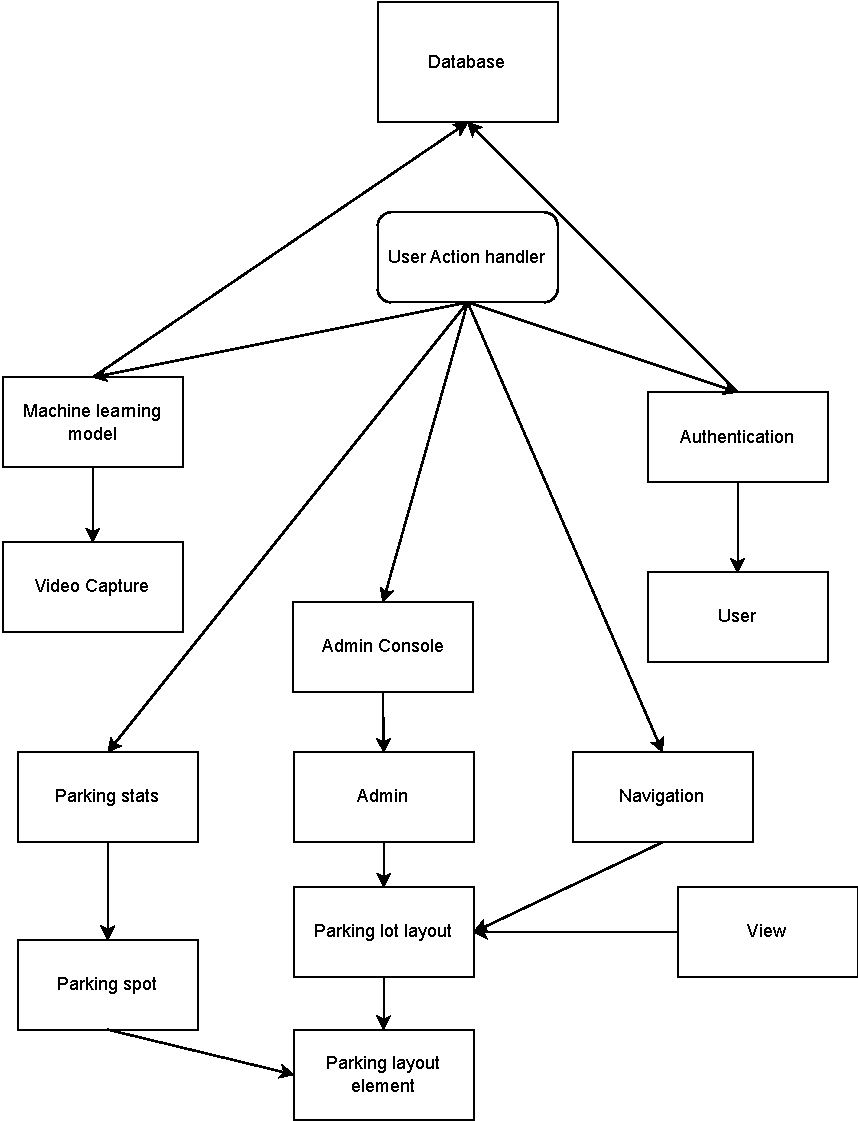
\includegraphics[width=0.9\textwidth]{UsesDiagram.pdf}
\caption{Use hierarchy among modules}
\label{FigUH}
\end{figure}

%\section*{References}

\newpage

\bibliographystyle {plainnat}
\bibliography{../../../refs/References}

\newpage{}

\end{document}